\documentclass[12pt]{article}

\usepackage{sbc-template}
\usepackage{graphicx,url}
\usepackage[utf8]{inputenc}
\usepackage[brazil]{babel}
\usepackage[T1]{fontenc}  
\usepackage{indentfirst}
\usepackage{graphicx}
\usepackage{float}
\usepackage[table,xcdraw]{xcolor}
\usepackage{tablefootnote}
     
    
\sloppy

\title{Krack Attack \\ An Study}

\author{Felipe A. C. Gemmal\inst{1}, Leonardo A. Basilio\inst{1},\\ João Gabriel S. Fernandes\inst{1}, Arthur C. Sousa\inst{1} }

\address{Instituto de Informática -- Universidade Federal do Goiás(UFG)\\
Alameda Palmeiras, Quadra D,Câmpus Samambaia -- \\ 74690-900 -- Goiânia -- GO -- Brazil 
 \email{\{felipegemmal,leonardobasilio,joaofernandes,arthursousa\}@inf.ufg.br}
}

\begin{document} 

\maketitle

\begin{abstract}
	This paper references the study of Krack Attack and its correlated components with the objective of completing the networks 2 graduation course in UFG.
\end{abstract}

\begin{resumo} 
	Esse artigo referencia o estudo do Krack Attack e seus componentes correlatos com o objetivo de completar o curso de graduação da UFG de redes 2.
\end{resumo}


%Tal pessoa escreve
\section{Introdução}
O \textit{Key Reinstallation Attacks}, apelidado de \textit{Krack Attacks} \cite{vanhoef:2017} foi desenvolvido em 2017 por Mathy Vanhoef do grupo de pesquisa DistriNet da universidade belga \textit{Ku Leuven}. Ele é um tipo de ataque ao sistema \textit{Wi-Fi}, mais precisamente ao protocolo WPA2 (\textit{Wi-Fi Protected Access}) responsável pela segurança da comunicação entre usuário e ponto de acesso. O ataque explora uma vulnerabilidade na etapa de autenticação, mais especificamente na parte de confirmação do \textit{4-way handshake}. Esse consiste na manipulação dos pacotes trocados entre as partes durante esta etapa, tornando-o um ataque do tipo \textit{Man in The Middle} (MITM).

Em dispositivos Android e Linux, que usam o cliente de \textit{Wi-Fi} \textit{wpa\_supplicant}, foi identificada uma situação específica em que a chave da sessão utilizada para criptografar os pacotes pode ser forçada pelo ataque a assumir o valor zero. Isso torna trivial interceptar e manipular o tráfego de dados entre esses dispositivos.

\section{Tecnologias envolvidas}
\subsection{\textit{Wi-Fi}}
É uma tecnologia criada para redes locais de rádio sem fio com dispositivos baseados no padrão IEEE 802.11. Dispositivos que completam com sucesso o teste de certificado de interoperabilidade podem ser chamados de \textit{Wi-Fi Certified} (Certificado em Wi-Fi). O padrão \textit{Wi-Fi} opera em faixas de frequências que não necessitam de licença para instalação e/ou operação. Dispositivos compatíveis podem acessar a internet por meio de uma rede local sem fio (WLAN) e um ponto de acesso sem fio. O \textit{Wi-Fi} geralmente opera nas faixas de 2,4 GHz e 5,8 GHz.

Tais ondas são influenciadas por vários materiais comuns, podendo ser refletidas ou absorvidas por estes, restringindo a distância de conexão do \textit{Wi-Fi}, mas esses também diminuem a interferência entre redes, pois como todas as redes sem fio são afetadas por interferências físicas, duas redes terão menos interferências entre si se houver estruturas físicas entre elas para refletir suas ondas.

Como o \textit{Wi-Fi} é uma rede sem fio, qualquer pessoa dentro da sua área de alcance com uma interface sem fio pode tentar acessá-la. Por isso, \textit{Wi-Fi} é mais vulnerável a ataques do que redes conectadas por fios.

\subsection{WPA2}
Também conhecido como IEEE 802.11i, é o sucessor do WPA, substituindo-o desde 2006. Ele traz melhorias de segurança ao protocolo \textit{Wi-Fi}, como a utilização do algoritmo de criptografia AES (\textit{Advanced Encryption Standard}) e a introdução de dois novos protocolos: \textit{4-way handshake} e \textit{group key handshake}. Porém, devido ao maior custo computacional deste protocolo, alguns equipamentos mais antigos podem ser incompatíveis com o WPA2.

\subsubsection{4-Way Handshake}
O \textit{4-way handshake} tem como função gerar um pequeno grupo de chaves de criptografia comuns entre as partes para o estabelecimento de uma conexão segura. O cliente \textit{Wi-Fi} e o ponto de acesso enviam mensagens um ao outro, que só podem ser descriptografadas com a chave de sessão PTK (\textit{Pairwise Transient Key}), que é derivada a partir da contatenação dos seguintes elementos: chave secreta compatilhada PMK (\textit{Pairwise Master Key}), ANonce (número único arbitrário, escolhido pelo ponto de acesso), SNonce (número único arbitrário, escolhido pelo cliente Wi-Fi), endereço MAC do ponto de acesso, endereço MAC do cliente \textit{Wi-Fi}. A PMK é derivada pela função PBKDF2-SHA1 (\textit{Password-Based Key Derivation Function 2}).

O esquema de funcionamento do protocolo se dá de acordo com as seguintes etapas: primeiro o ponto de acesso gera o ANonce e o envia para o cliente \textit{Wi-Fi} (mensagem 1/4), que irá derivar a chave PTK e enviar o seu número arbitrário (SNonce) junto de um MIC (\textit{Message Integrity Code}) (mensagem 2/4). Em seguida, o ponto de acesso também pode construir a chave PTK. Ele verifica a validade da mensagem 2 e constrói a chave GTK (\textit{Group Temporal Key}), se necessário, e a envia junto de outro MIC (mensagem 3/4) para o cliente \textit{Wi-Fi}, que verificará a validade da mensagem e responderá com uma confirmação ACK (mensagem 4/4).

Dessa forma, o \textit{4-way handshake} permite que tanto o cliente quanto o ponto de acesso possam provar um ao outro o conhecimento da chave PMK, sem nunca transmití-la pela rede, pois, se a descriptografia foi bem sucedida, então ambas as partes derivaram a mesma PTK (que depende da chave PMK).
    

\begin{figure}[H]
	\begin{center}
    	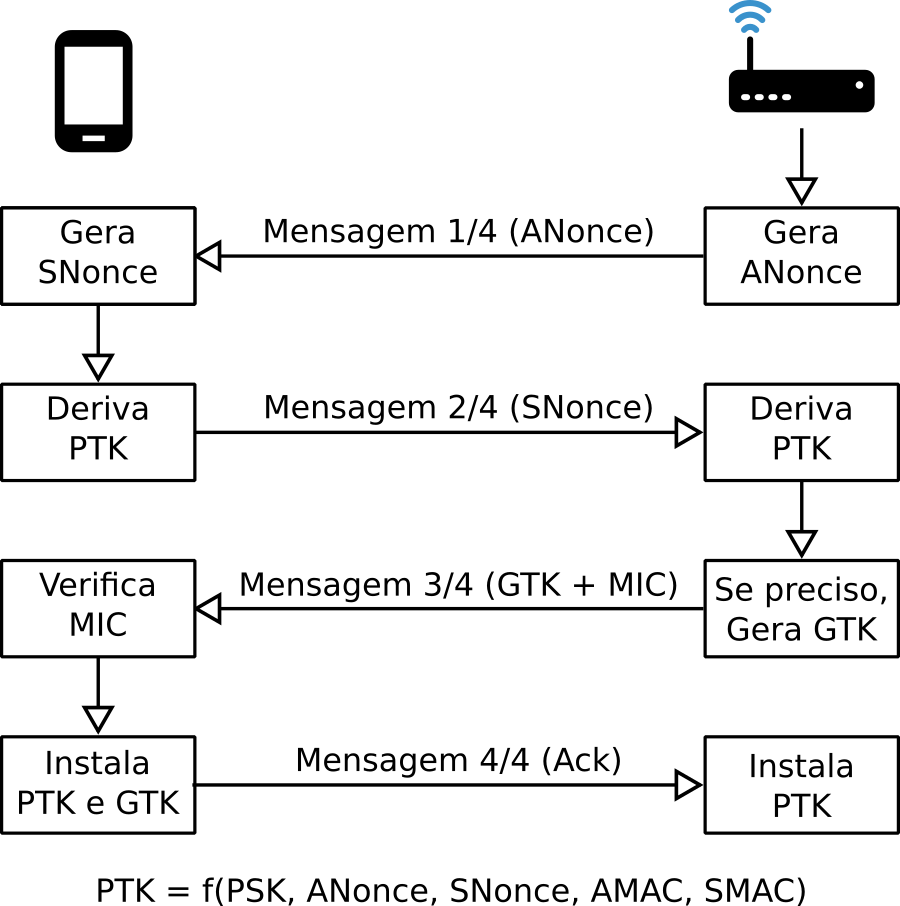
\includegraphics[width=12cm]{Handshake.png}
    	\caption{Diagrama de execução do \textit{4-way handshake}}
    	\label{fig:handshake}
	\end{center}		
\end{figure}

\subsection{O Ataque}

Para realizar o ataque, o atacante deve agir como um intermediario entre o dispositivo alvo e o roteador,  interceptando e encaminhando as mensagens enviadas entre eles e por isso necessita de duas interfaces de rede, uma para criar o ponto de acesso malicioso a que o dispositivo alvo conectar-se-á e outra para estabelecer conexão com o ponto de acesso original.

O ataque se inicia com um \textit{spoofing} de \textit{Wi-Fi} para forçar a conexão do cliente com o atacante. A imagem \ref{fig:ataque} mostra com mais detalhes como o ataque funciona. Esta se encontra no momento em que o \textit{4-way-handshake} é iniciado, após a comunicação inicial intermediada pelo atacante entre o dispositivo alvo e o ponto de acesso original. A troca de mensagens ocorre de forma esperada, mesmo com o atacante retransmitindo as mensagens, até que a quarta mensagem seja enviada pelo dispositivo alvo, quando será interceptada e bloqueada pelo atacante. Este então repetirá para o dispositivo alvo a terceira mensagem que foi anteriormente armazenada, levando o cliente a assumir que a quarta mensagem não foi entregada ao ponto de acesso original com sucesso. Neste momento, o dispositivo alvo então reinstalará sua chave PTK e transmitirá novamente a quarta mensagem. Em algumas implementações, a chave será reinstalada com o valor zero. A partir deste momento, como a chave será conhecida, a retransmissão de mensagens para o ponto de acesso original não é mais necessária, e o ponto de acesso malicioso poderá obter acesso total aos pacotes por ele trafegados.

\begin{figure}[H]
	\begin{center}
    	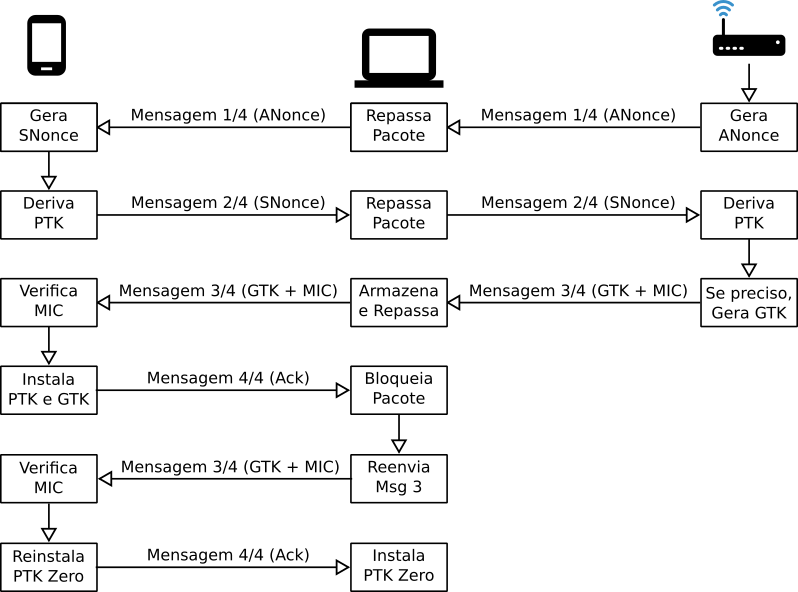
\includegraphics[width=15cm]{Ataque.png}
    	\caption{Diagrama de execução do \textit{4-way handshake}}
    	\label{fig:ataque}
	\end{center}		
\end{figure}

\subsection{Ferramenta}
O autor do ataque publicou um conjunto de \textit{scripts} desenvolvidos na linguagem Python que permitem a verificação da vulnerabilidade de qualquer implementação do \textit{4-way handshake}. Estes scripts estão disponíveis em um repositório no GitHub\footnote{https://github.com/vanhoefm/krackattacks-scripts}. Com eles é possível a realização de testes que exploram tanto a reinstalação da PTK quanto da GTK.

Embora o ataque destine-se à interceptação de dados sem a necessidade de se conhecer a senha da rede, para os testes é necessário que as credenciais sejam conhecidas. Isto porque o cliente alvo deve se conectar ao ponto de acesso que é emulado pelo \textit{script}. Este ponto de acesso é criado a partir de uma versão modificada do \textit{hostapd}, um serviço de espaço do usuário muito utilizado em sistemas Linux. Este serviço é executado e controlado a partir dos \textit{scripts} em Python. Pode-se usar tanto um SSID novo quanto um existente. Neste último caso, a rede é criada em um canal diferente do da original e o cliente é forçado a conectar-se à falsa rede.

Além disso, mesmo não disponibilizado no sítio do Krack, existe outro conjunto de \textit{scripts} que são uma prova de conceito para o caso partícular em que o ataque induz uma chave de sessão zerada (\textit{all zero key}). Com ele, é possível ter acesso aos pacotes criptografados que trafegam entre o aparelho vulnerável e o atacante, e como a chave é zerada todos os pacotes são facilmente legíveis.

Para a execução do ataque, é necessário que o computador que atuará como \textit{Man In The Middle} esteja equipado com duas interfaces \textit{Wi-Fi}, pois uma servirá como ponto de acesso para o aparelho vulnerável e a outra utilizada para se comunicar com o roteador de acesso original para o qual os pacotes iniciais do \textit{4-way handshake} serão redirecionados.


\section{Descrição do problema}
O caso do KrackAttacks que será abordado neste artigo diz respeito a um ato malicioso em que um cliente \textit{Wi-Fi} Android ou Linux é induzido a mudança da chave de criptografia de sessão para zero (\textit{all zero key}). Isso é feito manipulando-se o processo de \textit{4-way-handshake} entre um cliente e um ponto de acesso, mais especificamente após a terceira mensagem, quando é instalada uma chave, e caso uma resposta de confirmação não seja recebida, a terceira mensagem será reenviada e a chave reinstalada. Foi mostrado que um ataque pode forçar essas reinstalações da chave com uma coleta e repetição da terceira mensagem. 

Caso o ataque ocorra com sucesso, o atacante tem a capacidade de interferir em todas as trocas entre cliente e ponto de acesso, podendo assim: alterar dados de compras, ter acesso a dados pessoais, informações de cartão de crédito, redirecionar os pedidos de conexão para um sítio malicioso e alterar pacotes recebidos pelo cliente para softwares maliciosos. 

Note que tal ataque não pode resultar na obtenção da senha da rede utilizada, nem das chaves de criptografia usadas para o \textit{handshake}. Também não é possível descriptografar pacotes criptografados, e como a grande maioria da troca de pacotes em rede é criptografada, pode ser necessária a combinação deste ataque com outras técnicas, para que se obtenha melhores resultados.


\section{Proposta de experimento}
O objetivo do experimento é reproduzir o ataque demonstrado em vídeo\footnote{https://www.youtube.com/watch?v=Oh4WURZoR98} pelo autor. Considerando-se que no sítio oficial do ataque foram disponibilizados somente os \textit{scripts} de teste da vulnerabilidade, fazia-se necessário implementar o ataque para o caso particular da \textit{all zero key} utilizando estes \textit{scripts} como base. Para isso, algoritmos e técnicas como \textit{Wi-Fi spoofing} seriam modificados e inseridos a fim de que se pudesse capturar os pacotes ao se agir como um intermediário para o cliente. Porém, durante os estudos foi encontrado o \textit{script} feito pelo próprio autor que realiza o ataque com a chave zero. Então, optou-se por entendê-lo e utilizá-lo no lugar de se realizar uma nova implementação.  

Além disso, dada a alegação do autor de que, à época da descoberta da vulnerabilidade, cerca de 50\% dos aparelhos Android encontravam-se vulneráveis ao ataque, decidiu-se realizar um levantamento com os estudantes do Instituto de Informática (INF), com o objetivo de se identificar qual o pertecentual atual ainda vulnerável ao ataque após 1 ano de sua publicação. Registrando marcas, modelos e versões do sistema operacional de aparelhos celulares Android, será compilada uma tabela com os dados obtidos.

\section{Realização do experimento}
Para a preparação do cenário propício para o experimento, foram necessárias algumas etapas. Primeiro foi necessário a identificação de um aparelho celular vulnerável ao ataque com o auxilio do \textit{script} de teste. Para este experimento foi utilizado o Phoenix 4.0 do fabricante IPRÓ com versão Android 6.0.

O \textit{script} de ataque tem como requisito um ponto de acesso alvo e duas interfaces (no atacante) \textit{Wi-Fi}, para que se possa fazer o roteamento conforme explicado na sessão que descreve o ataque. Neste caso o ponto de acesso utilizado foi o D-Link DIR-610N.


\section{Resultados do experimento}
Para o levantamento proposto, foi avaliada uma amostra de 23 aparelhos celulares. Os resultados podem ser vistos na Tabela \ref{table:Tabela1}. Observamos que cerca de 84\% dos aparelhos analisados não são vulneráveis ao ataque em contraste com os 50\% alegados pelo autor. Nota-se que, assim como afirmado no artigo do autor, a vulnerabilidade predomina a partir da versão Android 6.0. Outro fator de influência é o fabricante. Dentre os analisados só foram encontradas vulnerabilidades nas marcas Asus e Lenovo. Porém no Asus observamos que a falha foi corrigida com as atualizações mais recentes do sistema Android. 

\begin{table}[H]
\caption{Resultado da avaliação de vulnerabilidade}
\begin{tabular}{|c|c|c|c|c|}
\hline

\textbf{Fabricante} & \textbf{Modelo}   & \textbf{Sistema Operacional} & \multicolumn{1}{l|}{\textbf{Quantidade}} & \textbf{Vulnerabilidade} \\ \hline
Motorola            & Moto Z- 1ªGeração & Android 8.0.0                & 3                                        & Não Vulnerável           \\ \hline
Asus                & Zenfone 4 Selfie  & Android 8.1.0                & 1                                        & Não Vulnerável           \\ \hline
Asus                & Zenfone 4 Selfie  & Android 7.1.0                & 1                                        & Vulnerável               \\ \hline
LG                  & L20 D100          & Android 4.4.0                & 1                                        & Não Vulnerável           \\ \hline
Motorola            & Moto E            & Android 7.1.0                & 2                                        & Não Vulnerável           \\ \hline
Xiaomi              & Redmi             & Android 7.0.0                & 1                                        & Não Vulnerável           \\ \hline
Motorola            & Moto G5           & Android 8.1.0                & 3                                        & Não Vulnerável           \\ \hline
Samsung             & S7                & Android 7.0.0                & 4                                        & Não Vulnerável           \\ \hline
Asus                & Zenfone 3 Max     & Android 8.1.0                & 2                                        & Não Vulnerável           \\ \hline
Asus                & Zenfone 3 Max     & Android 7.0.0                & 1                                        & Vulnerável               \\ \hline
Lenovo              & Vibe K6           & Android 7.0.0                & 1                                        & Vulnerável               \\ \hline
Positivo            & Twist S520        & Android 6.1.0                & 1                                        & Não Vulnerável           \\ \hline
Samsung             & J2                & Android 5.1.0                & 2                                        & Não Vulnerável           \\ \hline
\rowcolor[HTML]{FCFF2F} 
IPRÓ                & Phoenix 4.0\tablefootnote{Aparelho utilizado no experimento}      & Android 6.0.0                & 1                                        & Vulnerável               \\ \hline
\end{tabular}
\label{table:Tabela1}
\end{table}


O experimento de ataque foi realizado com sucesso. Pôde-se vizualizar a troca de mensagens que não eram criptografadas pela camada de aplicação. Porém, para as que eram, foi necessário o uso de outras ferramentas, como \textit{sslstrip}, para sua remoção.



%\textit{arp spoofing}


%\section{Conclusão}


%\begin{abstract}
%  This meta-paper describes the style to be used in articles and short papers
%  for SBC conferences. For papers in English, you should add just an abstract
%  while for the papers in Portuguese, we also ask for an abstract in
%  Portuguese (``resumo''). In both cases, abstracts should not have more than
%  10 lines and must be in the first page of the paper.
%\end{abstract}
     
%
%
%\section{General Information}
%
%All full papers and posters (short papers) submitted to some SBC conference,
%including any supporting documents, should be written in English or in
%Portuguese. The format paper should be A4 with single column, 3.5 cm for upper
%margin, 2.5 cm for bottom margin and 3.0 cm for lateral margins, without
%headers or footers. The main font must be Times, 12 point nominal size, with 6
%points of space before each paragraph. Page numbers must be suppressed.
%
%Full papers must respect the page limits defined by the conference.
%Conferences that publish just abstracts ask for \textbf{one}-page texts.
%
%\section{First Page} \label{sec:firstpage}
%
%The first page must display the paper title, the name and address of the
%authors, the abstract in English and ``resumo'' in Portuguese (``resumos'' are
%required only for papers written in Portuguese). The title must be centered
%over the whole page, in 16 point boldface font and with 12 points of space
%before itself. Author names must be centered in 12 point font, bold, all of
%them disposed in the same line, separated by commas and with 12 points of
%space after the title. Addresses must be centered in 12 point font, also with
%12 points of space after the authors' names. E-mail addresses should be
%written using font Courier New, 10 point nominal size, with 6 points of space
%before and 6 points of space after.
%
%The abstract and ``resumo'' (if is the case) must be in 12 point Times font,
%indented 0.8cm on both sides. The word \textbf{Abstract} and \textbf{Resumo},
%should be written in boldface and must precede the text.
%
%\section{CD-ROMs and Printed Proceedings}
%
%In some conferences, the papers are published on CD-ROM while only the
%abstract is published in the printed Proceedings. In this case, authors are
%invited to prepare two final versions of the paper. One, complete, to be
%published on the CD and the other, containing only the first page, with
%abstract and ``resumo'' (for papers in Portuguese).
%
%\section{Sections and Paragraphs}
%
%Section titles must be in boldface, 13pt, flush left. There should be an extra
%12 pt of space before each title. Section numbering is optional. The first
%paragraph of each section should not be indented, while the first lines of
%subsequent paragraphs should be indented by 1.27 cm.
%
%\subsection{Subsections}
%
%The subsection titles must be in boldface, 12pt, flush left.
%
%\section{Figures and Captions}\label{sec:figs}
%
%
%Figure and table captions should be centered if less than one line
%(Figure~\ref{fig:exampleFig1}), otherwise justified and indented by 0.8cm on
%both margins, as shown in Figure~\ref{fig:exampleFig2}. The caption font must
%be Helvetica, 10 point, boldface, with 6 points of space before and after each
%caption.
%
%\begin{figure}[ht]
%\centering
%\includegraphics[width=.5\textwidth]{fig1.jpg}
%\caption{A typical figure}
%\label{fig:exampleFig1}
%\end{figure}
%
%\begin{figure}[ht]
%\centering
%\includegraphics[width=.3\textwidth]{fig2.jpg}
%\caption{This figure is an example of a figure caption taking more than one
%  line and justified considering margins mentioned in Section~\ref{sec:figs}.}
%\label{fig:exampleFig2}
%\end{figure}
%
%In tables, try to avoid the use of colored or shaded backgrounds, and avoid
%thick, doubled, or unnecessary framing lines. When reporting empirical data,
%do not use more decimal digits than warranted by their precision and
%reproducibility. Table caption must be placed before the table (see Table 1)
%and the font used must also be Helvetica, 10 point, boldface, with 6 points of
%space before and after each caption.
%
%\begin{table}[ht]
%\centering
%\caption{Variables to be considered on the evaluation of interaction
%  techniques}
%\label{tab:exTable1}
%\includegraphics[width=.7\textwidth]{table.jpg}
%\end{table}
%
%\section{Images}
%
%All images and illustrations should be in black-and-white, or gray tones,
%excepting for the papers that will be electronically available (on CD-ROMs,
%internet, etc.). The image resolution on paper should be about 600 dpi for
%black-and-white images, and 150-300 dpi for grayscale images.  Do not include
%images with excessive resolution, as they may take hours to print, without any
%visible difference in the result. 
%

\section{Referências}

%
%Bibliographic references must be unambiguous and uniform.  We recommend giving
%the author names references in brackets, e.g. \cite{knuth:84},
%\cite{boulic:91}, and \cite{smith:99}.
%
%The references must be listed using 12 point font size, with 6 points of space
%before each reference. The first line of each reference should not be
%indented, while the subsequent should be indented by 0.5 cm.
%
\bibliographystyle{sbc}
\bibliography{sbc-template}

\end{document}
